\chapter{Попередні роботи присвячені співставленню точкових множин}

В першому розділі розглянуто коротку історію досліджень,
що пов'язані зі співсталенням точкових множин
за допомогою ітеративного алгоритму найближчих точок.
Розбір попередніх робіт дає змогу чітко поставити задачу,
що розв'язується в другому та третьому розділах дипломної роботи.

\section{Перші описи алгоритму}

У лютому 1992 року Пол Бесл та Ніл Маккей опублікували статтю з описом
ітеративного алгоритму найближчих точок для співставлення точкових множин
\cite{besl:mckey}.
Алгоритм полягає в ітеративній мінімізації середньоквадратичної відстані між
тривимірними множинами.
В роботі доведено, що алгоритм монотонно збігається до локального мінімуму цієї
метрики.

У квітні 1992 року Ян Чен та Жерар Медіоні опубліковали статтю,
в якій описали застосування ітеративного алгоритму найближчих точок
для отримання повної моделі фізичного об'єкта \cite{chen:medioni}.
Результати роботи представлені на прикладі реконструкції гіпсового зубу та
бюсту Моцарта (рис. \ref{fig:mozart}).
На перших двох рисунках зображені дві вхідні множини,
на третьому~---~результат роботи алгоритму.

\begin{figure}[h]
  \centering
    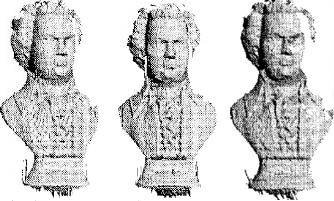
\includegraphics[width=0.9\textwidth]{images/mozart}
  \caption{Бюст Моцарта}
  \label{fig:mozart}
\end{figure}

\section{Сучасні роботи}

На момент написання дипломної роботи одними з новітніх робіт,
де був використаний ітеративний алгоритм найближчих точок,
є перевірка правильності положення пацієнта на томотерапії при лікуванні
онкологічних захворювань \cite{radiotherapy} та виявлення геометричних
деформацій стін, стелі та доріг підземної парковки,
за якими ведеться спостереження \cite{infractructure}.
В останній статті розв'язується задача одночасної локалізації і картографування
всередині будівлі, де неможливо використовувати GPS.

\section{Постановка задачі}

Запишемо постановку задачі, яка досліджується у згадуваних статтях.
Є дві множини:
вихідна $S \subset \mathbb{R}^3$ та цільова $T \subset \mathbb{R}^3$.
Точки вихідної множини $ \boldsymbol{s} \in S$ повернули за допомогою матриці
\begin{equation*}
  \begin{cases}
    R \in \mathbb{R}^{3 \times 3}, \\
    R^T = R^{-1}, \\
    \det{R} = 1
  \end{cases}
\end{equation*}
та зсунули за допомогою вектора $ \boldsymbol{b} \in \mathbb{R}^3$.
Також в процесі сканування
з'явився адитивний ґаусів шум з незалежними компонентами на невідомою дисперсією
\begin{equation}\label{eq:problem}
  \boldsymbol{k_s} = R \cdot \boldsymbol{s} + \boldsymbol{b} + \boldsymbol{ \xi_s}, \qquad
  \boldsymbol{ \xi_s } \sim N \left( \boldsymbol{0}, \sigma^2 \cdot I \right),
\end{equation}
де $k \, : \, S \to T$~---~розмітка, тобто сюр'єктивне відображення,
яке співставляє кожну точку вихідної множини з точкою з цільової множини.

Задача полягає в такому виборі матриці $R$ та вектора $ \boldsymbol{b}$,
за яких евклідова відстань між $ \boldsymbol{k_s}$ та $R \cdot \boldsymbol{s} + \boldsymbol{b}$ для
всіх $ \boldsymbol{s} \in S$ була б найменшою.

\section{Модифікації}

В деяких роботах \cite{Hao:Li, nicp} при оптимізації враховують не тільки точки
двох множин, але й нормалі до них, а також відстані між деякими точками
множать на ваги.

\section*{Висновки до розділу 1}
\addcontentsline{toc}{section}{Висновки до розділу 1}

Проведено огляд задач, при розв'язанні яких використовується ітеративний
алгоритм найближчих точок.
Поставлена задача, розв'язання якої наведено в наступних розділах
дипломної роботи.
